须弥沙漠有许多山,这些山大都无法攀爬,让旅行者感觉很不方便。

众所周知,蒙德城的温迪曾经削掉了蒙德的山头丢进海里以平整地块,并形成了金苹果群岛。

然而温迪不能削掉这些山头,但是他可以帮助你完成\textbf{至多一次}上山。

这些山头都可以被近似认为是多边形,如下图所示,最短路的顶点一定在障碍物多边形的顶点上。

\begin{center}
  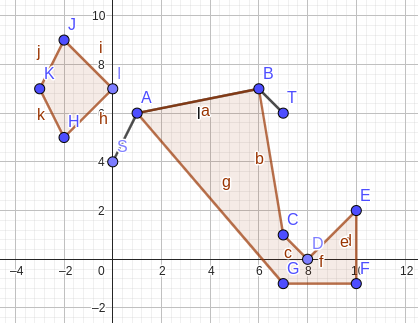
\includegraphics[scale=0.8]{example.png} \\
  \small{一条从$S$到$T$的最短路}
\end{center}

温迪觉得这道题对你来说太难了,所以他帮你处理了几何关系,确切地说,他将告诉你起点,终点,各个多边形的顶点之间是所有无需上山可达的点对,恰好一次上山可达的点对,以及这些点对之间的距离。

看不懂没关系,形式化地,给出一个有红蓝两种边的无向带权图,求至多经过一条蓝边的从起点到终点的最短路。或者断言无论如何都无法到达终点。

\begin{center}
  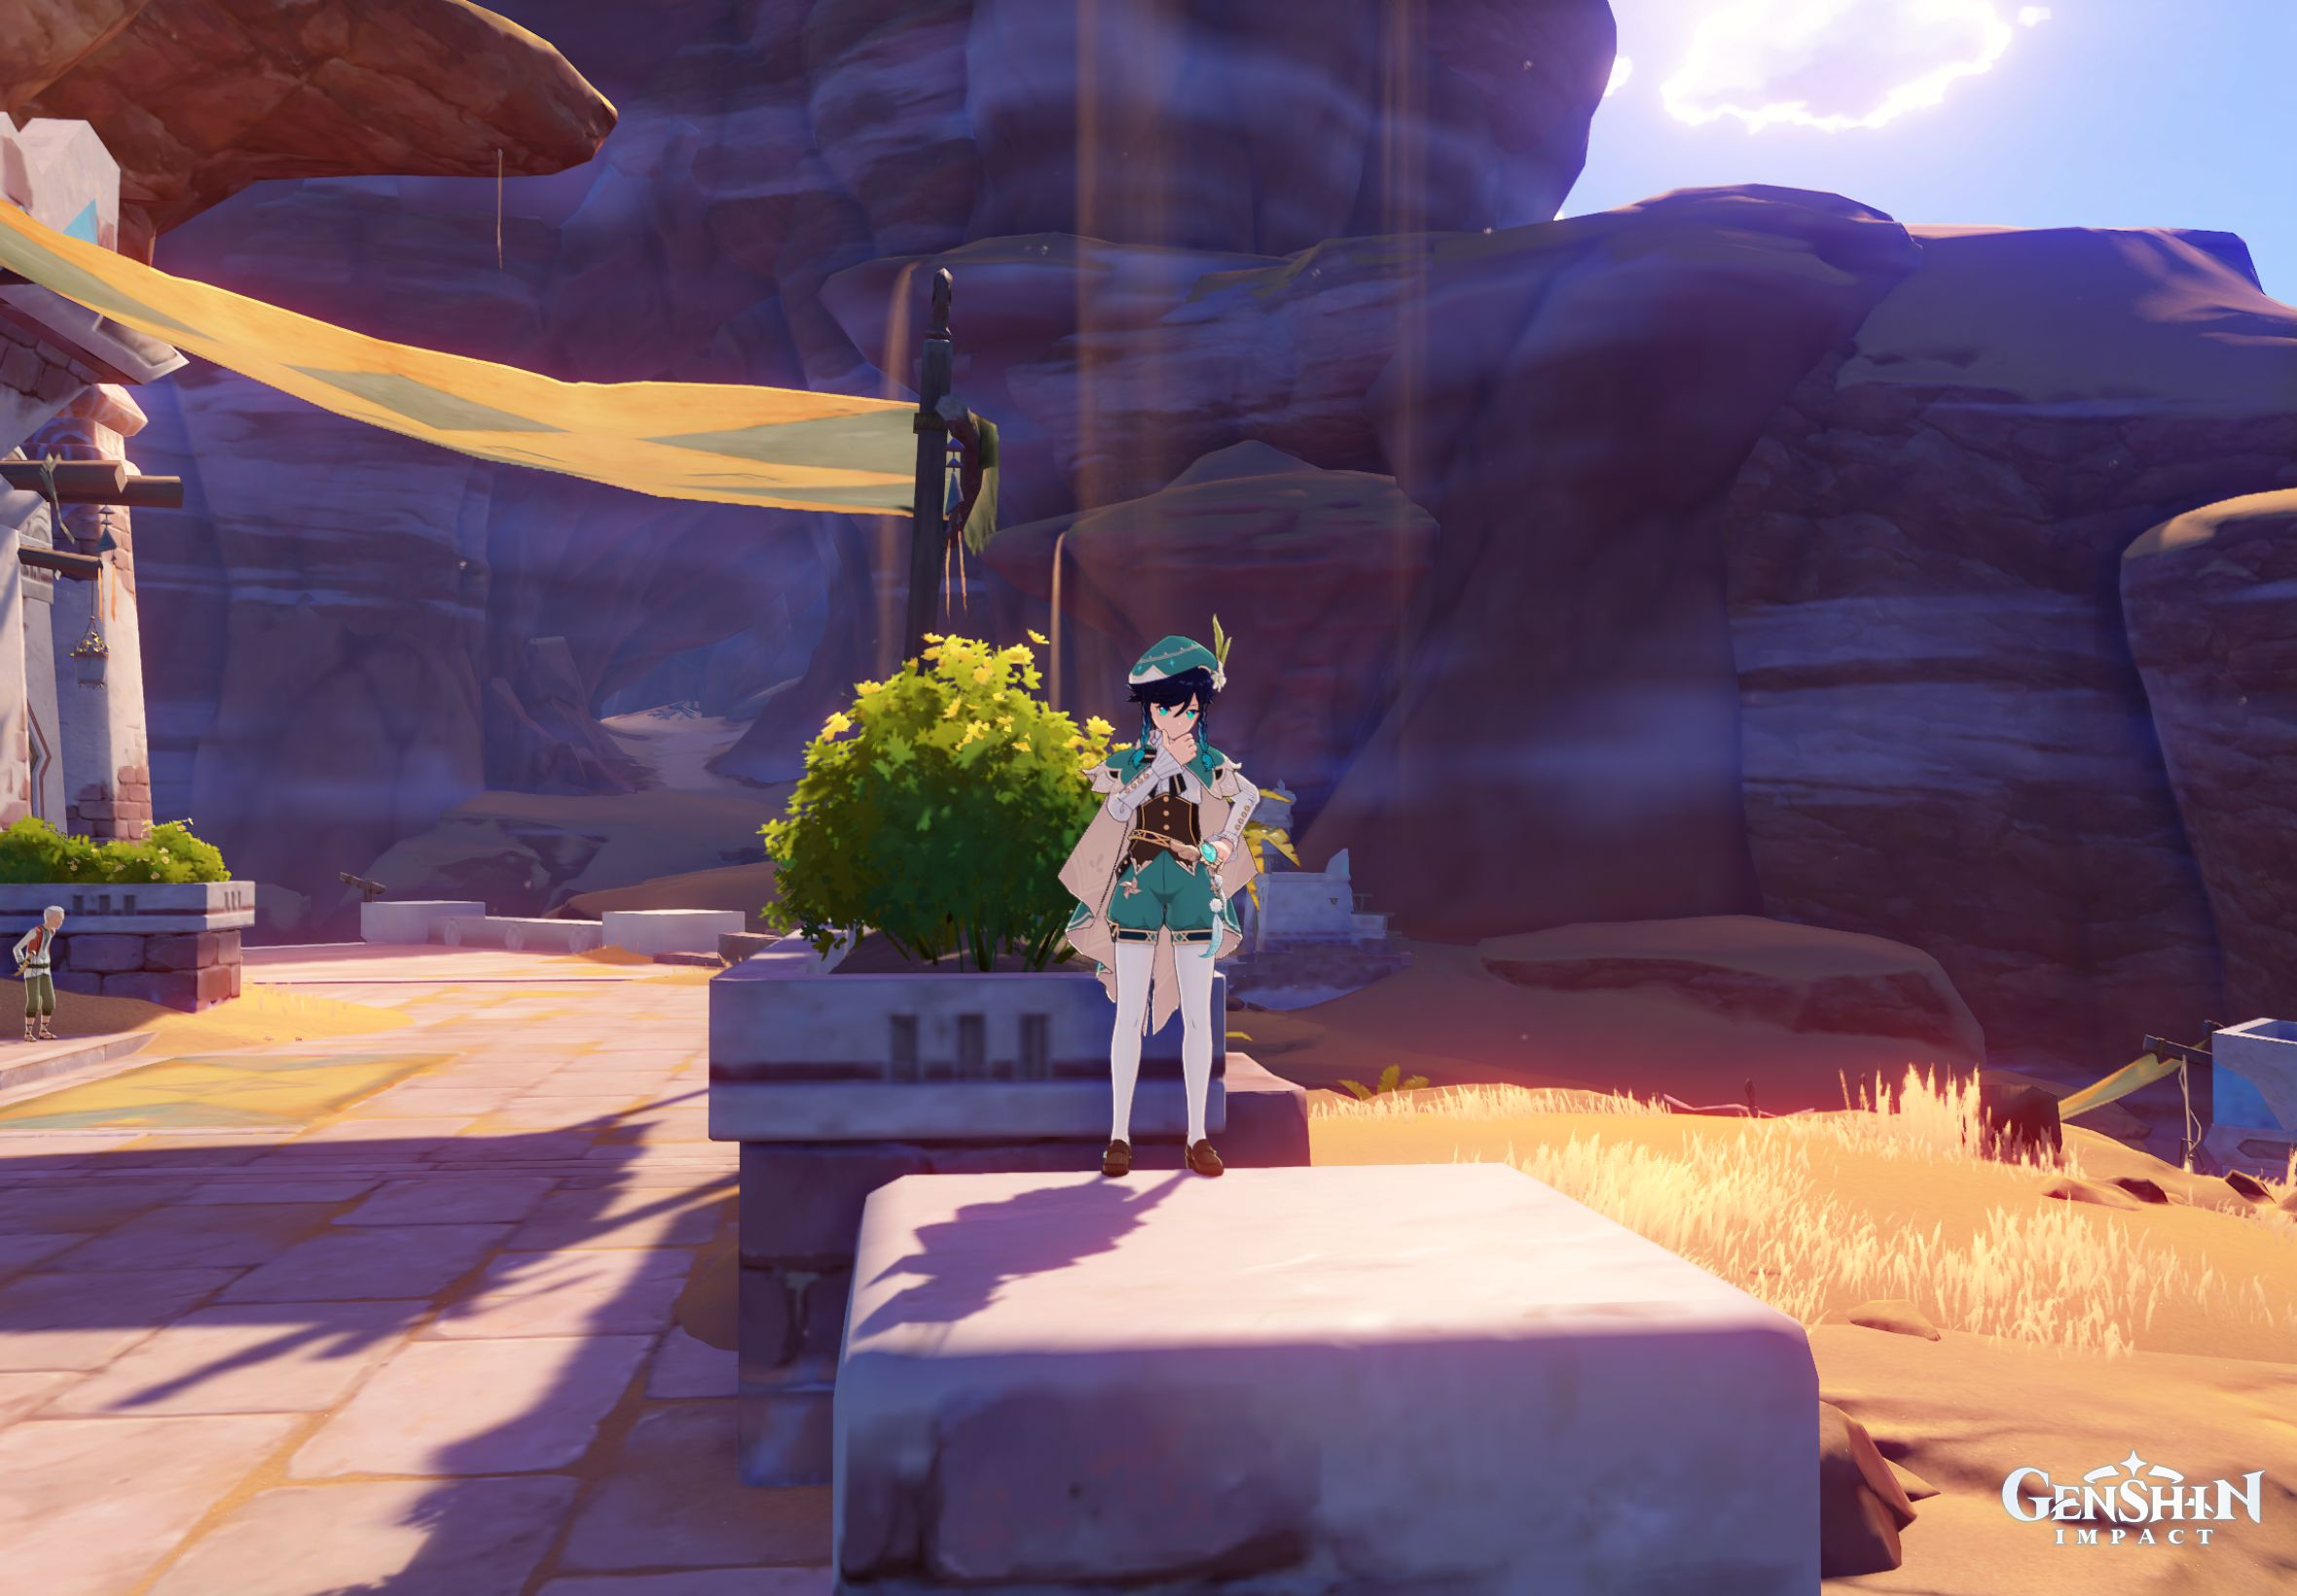
\includegraphics[scale=0.15]{venti.jpg} \\
  \small{温迪可爱!}
\end{center}
